%*******************************************************************************
%*********************************** First Chapter *****************************
%*******************************************************************************

\chapter{Plastic deformation by dislocation motion}  %Title of the First Chapter


\graphicspath{{Chapter1/Figs/Vector/}{Chapter1/Figs/Raster/}{Chapter1/Figs/PDF/}{Chapter1/Figs/}}


Dislocation motion is important in crystalline materials. In many metals, particularly those with an face-centred cubic structure such as copper or aluminium, dislocations must be hindered to achieve useful strength as an engineering material. Much of physical metallurgy is the study of the microstructural features that affect dislocation motion and their genesis in materials processing or alloys composition.

In other materials the crystal structure itself provides such a large barrier to motion that almost no plastic deformation is possible and these materials usually fail by brittle fracture. This is true of many non-metallic materials widely used as protective coatings or as functional materials in devices. Fracture is often the life limiting factor for these materials such that if their toughness was increased by making plastic flow were easier their lifetime would be extended. 

Even in some metallic materials with comparatively simple crystal structures plastic flow is limited not by microstructural features but by the inherent resistance of the crystal structure to the motion of dislocations. The ductile to brittle transition in many metals is due to the lattice resistance, notably iron in its body-centred crystal structure becomes brittle at low temperatures resulting in the infamous failure of the liberty ships during the second world war in the cold waters of the north Atlantic; originally thought to be due to high stresses caused by the (then novel) welding technique used to join the steel, it was Dr Constance Tipper who showed that it was the lack of plastic flow around the crack tip that allowed for the catastrophic fracture of entire ships \cite{Cottrell1997}. 

Thus there is a great motivation to understanding the inherent resistance to dislocation flow in a crystal structure, or \emph{lattice resistance}, and to being able to alter that lattice resistance and thereby introduce toughness to otherwise brittle phases.


%********************************** %First Section  **************************************
\section{Dislocations} %Section - 1.1 

Dislocations are line defects in crystals that are important for many reasons but in the context of the current work principally because they mediate plastic deformation. In the early twentieth century there were many observations of real world materials strengths that could not be reconciled with the theoretical shearing strength of a perfect plane of atoms. Indeed for a long time this was neglected because, as \citet{gordon1991} puts it:
\begin{quote}
``Until about 1934 the Establishment explanation of these phenomena was remarkably unconvincing and seems to have reflected mainly a desire not to be asked embarrassing questions.''
\end{quote}

In 1934 the edge dislocation was proposed by \citet{orowan1934i,orowan1934ii,orowan1934iii}, \citet{Taylor1934}, and \citet{polanyi1934} to explain the discrepancy between the ideal strength of crystal and the observed strengths of real materials. It was around this time that work undertaken by \citet{Volterra1907} and others %% Cite some here
on elastic behaviour of homogeneous isotropic continua was related to plastic flow of crystalline materials and indeed idealised dislocations in elastic continua are termed Volterra dislocations. By the end of the decade \citet{burgers1939} had described screw dislocations.

It was not until the 1950s that experimental evidence for the existence of dislocations was produced ; the principle evidence at that time being growth surfaces of single crystals, preferential etching of a crystalline material at dislocations and x-ray studies of arrays of dislocations in the bulk \cite{Forty1954}. 

Growth surfaces provide evidence for dislocations because, as \citet{Frank1949} predicted in 1949, a step could terminate by the intersection of a dislocation with a free surface, or conversely a dislocation intersecting with a free surface would necessarily create a step. The observation of such steps was very soon after Frank's prediction in 1950 by \citet{Griffin1950}.

Etch pits were shown to form at the intersections between dislocations and free surfaces by \citet{Horn1952} who observed that the configuration of etch pits matched the pre-existing surface growth features that arise from screw dislocations.

Arrays of dislocations can be detected by x-ray methods. The observation of Laue spots of an single crystal through the processes of plastic deformation and what we now call recovery provided indirect evidence for the existence of dislocation arrays. The process, described by \citet{Cottrell1949}, is as follows: Initially sharp Laue spots exist for a relatively perfect single crystal. These spots are then smeared during the process of plastic deformation which creates large numbers of dislocations throughout the crystal. The spots then split into distinct sharp spots during the process of recovery by which annealing allows dislocations to align into arrays and thereby minimise the elastic strain energy. These arrays form sub-grains, regions of perfect (or at least relatively perfect) crystal separated by low angle boundaries formed by arrays of dislocations.


\subsection{The stress required to move a dislocation}

Though mathematical descriptions of dislocations in isotropic elastic continua date back to 1907 \cite{Volterra1907} the energies and forces around dislocations in crystalline lattices was not considered until much later. In 1940 \citet{Dehlinger1940} and \citet{Peierls1940}. The former presented the application of the Frenkel-Kontorova model, a one dimensional array of balls connected by springs on a periodic potential/substrate, to approximate a dislocation.

The latter, Rudolph Peierls, was one of the physicists working during the great advent of quantum mechanics and most of his work was in that field, he was lectured by Planck, he worked with Pauli, Landau and others and
notably developed the idea of zones in the physics of phonons before Léon Brillouin and the statistical mechanics of alloys which formed the basis of mean-field theories for structural phase changes.
However during his education he received a grounding in classical physics at Arnold Sommerfeld's lectures in Munich and so it was that he was suitably equipped when presented with the problem of dislocation motion by Egon Orowan; as Peierls remarked he knew nothing about dislocation but he did know classical elasticity \cite{Edwards1996}.


Peierls presented the first formal solution for the dislocation displacement potential in a rather short note \cite{Peierls1940} and the idea was extended by \citet{Nabarro1947}. The model is remarkably simple; consider two semi-infinite perfect crystals with their lattice aligned but some initial misalignment between them as shown in \autoref{fig:semi_infinite_crystals}. We can join them along what will become the slip plane. An edge dislocation is formed where the energy of the system is lowered by displacing atoms from their initial positions to localise the misalignments around the dislocation core, usually taken to be the origin. I.e. when the energy of a planar defect is higher than that of the linear defect and dislocation will form.


\begin{figure}
\centering

    \begin{subfigure}{0.4\textwidth}
        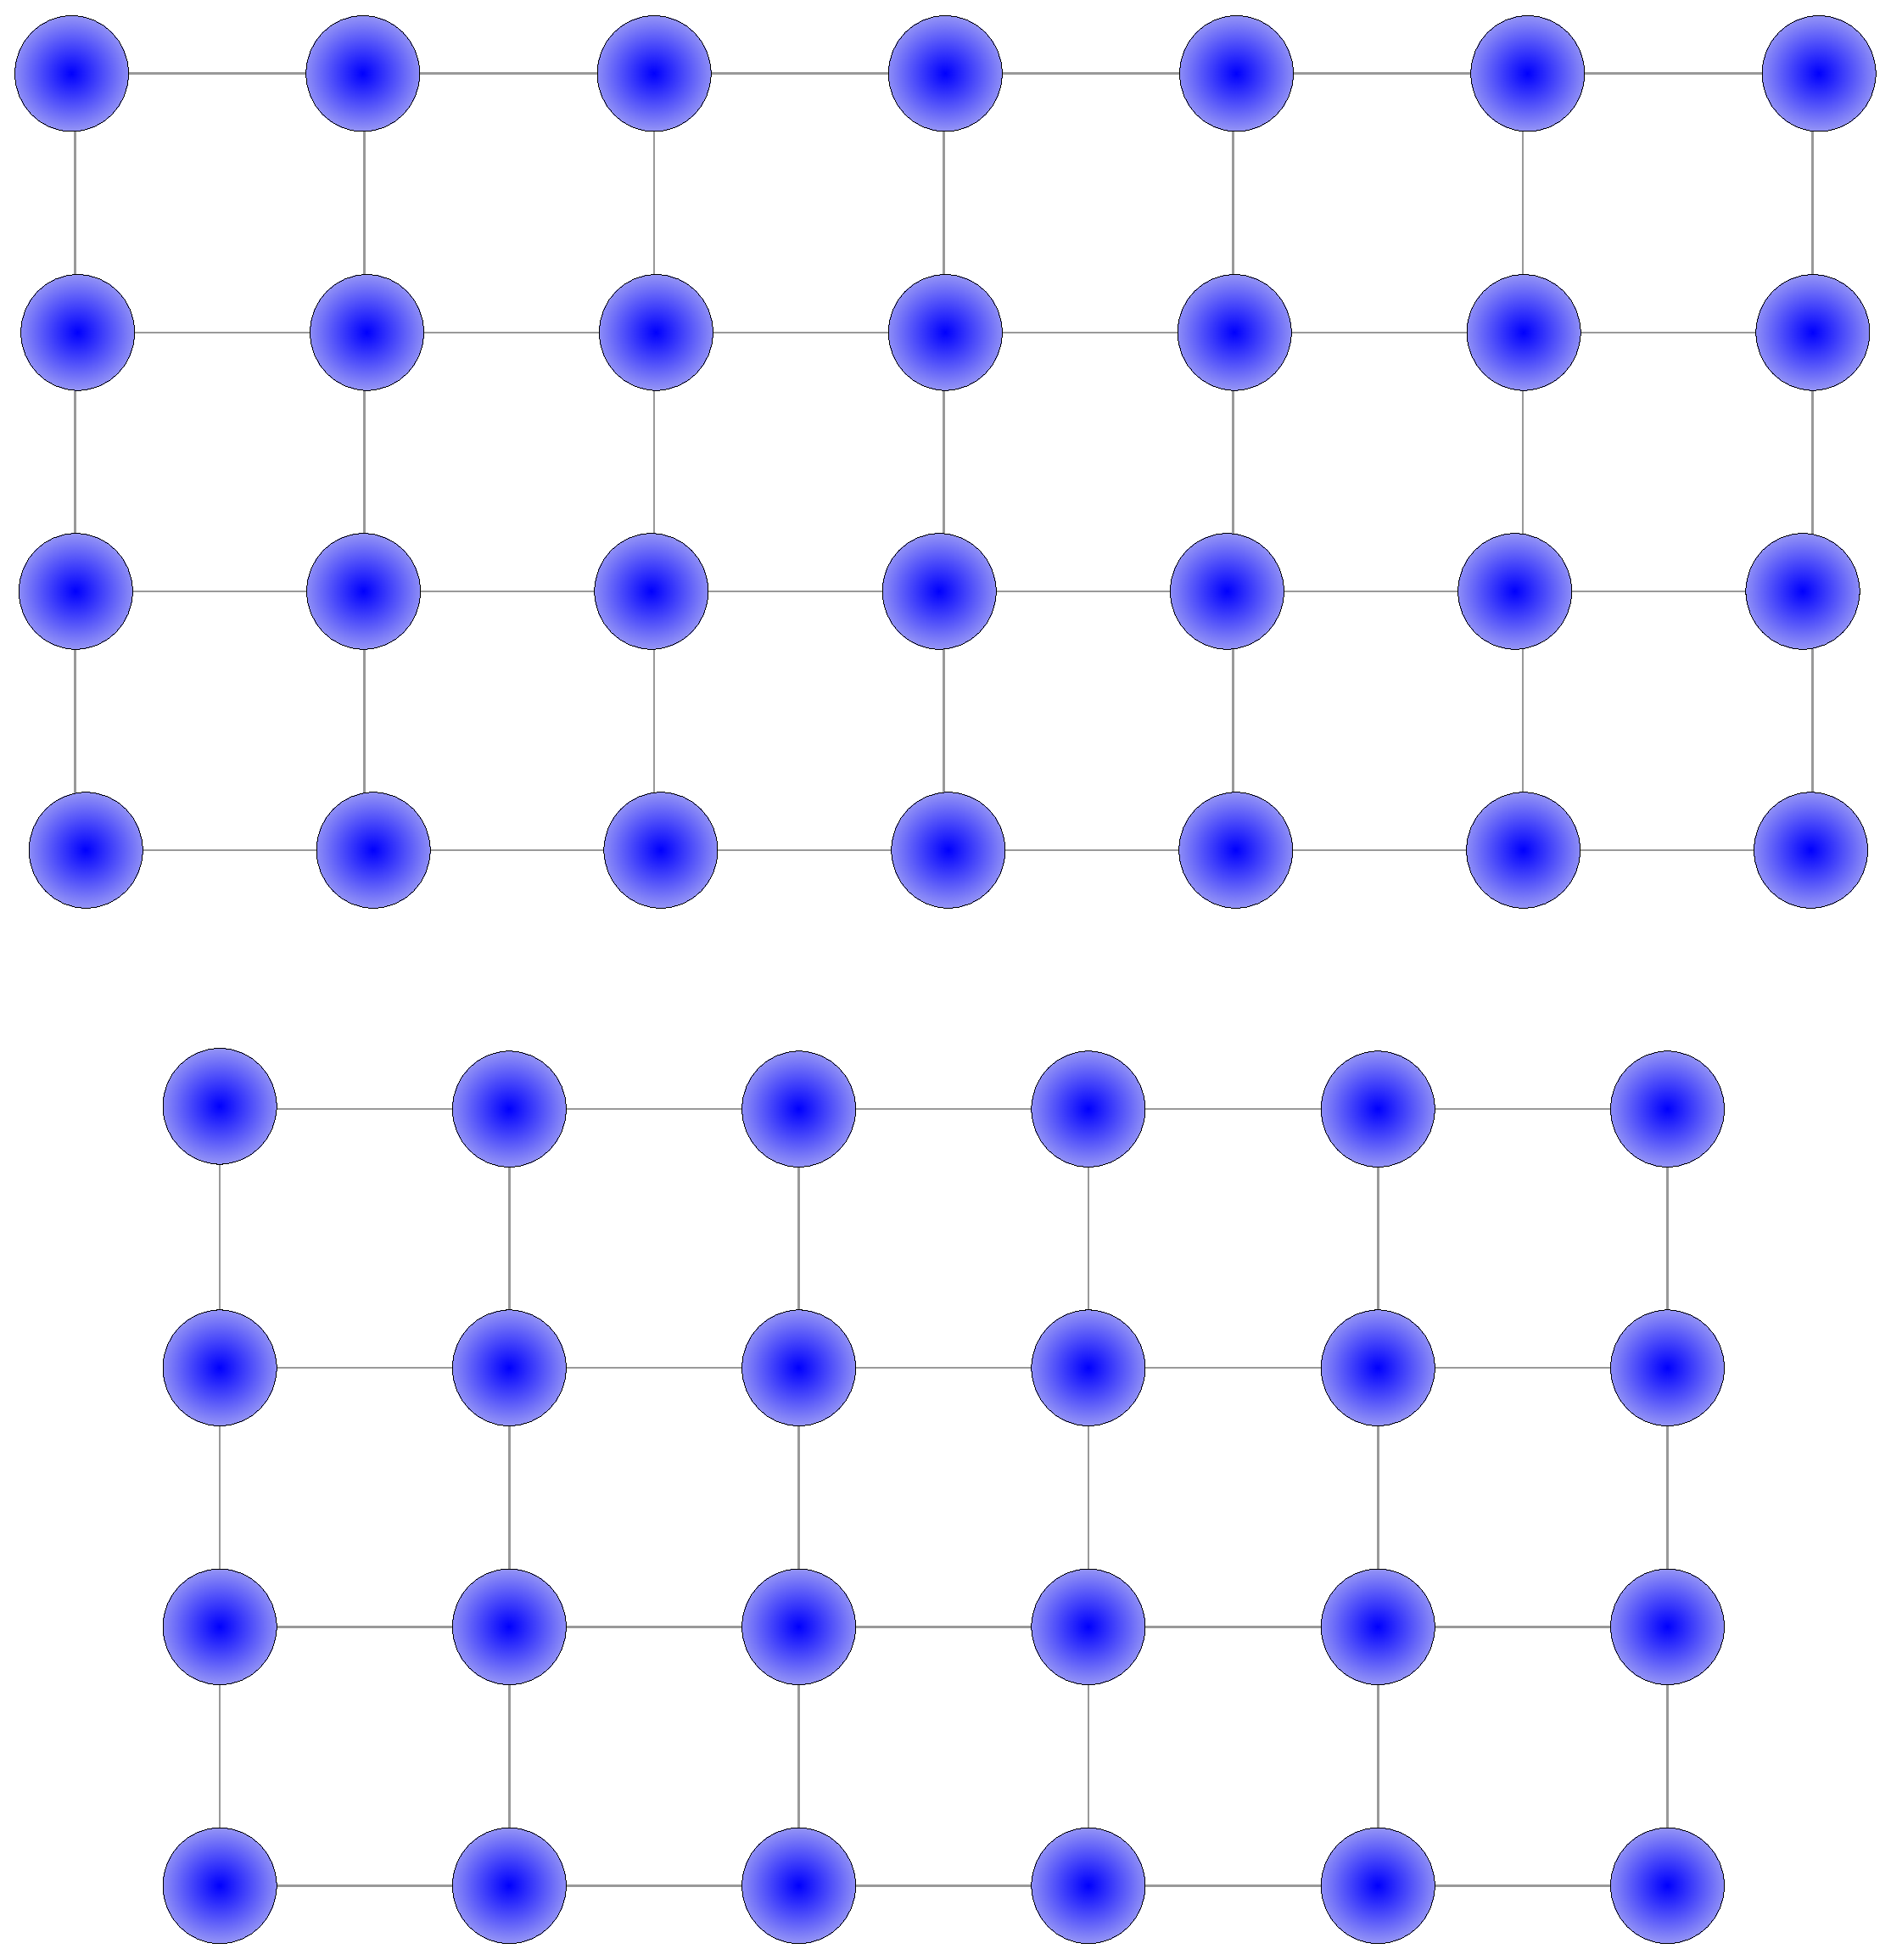
\includegraphics[width=\textwidth]{Half_crystals}
        \caption{Two semi-infinite crystals \label{fig:semi_infinite_crystals}}
    \end{subfigure}

    \begin{subfigure}{0.4\textwidth}
        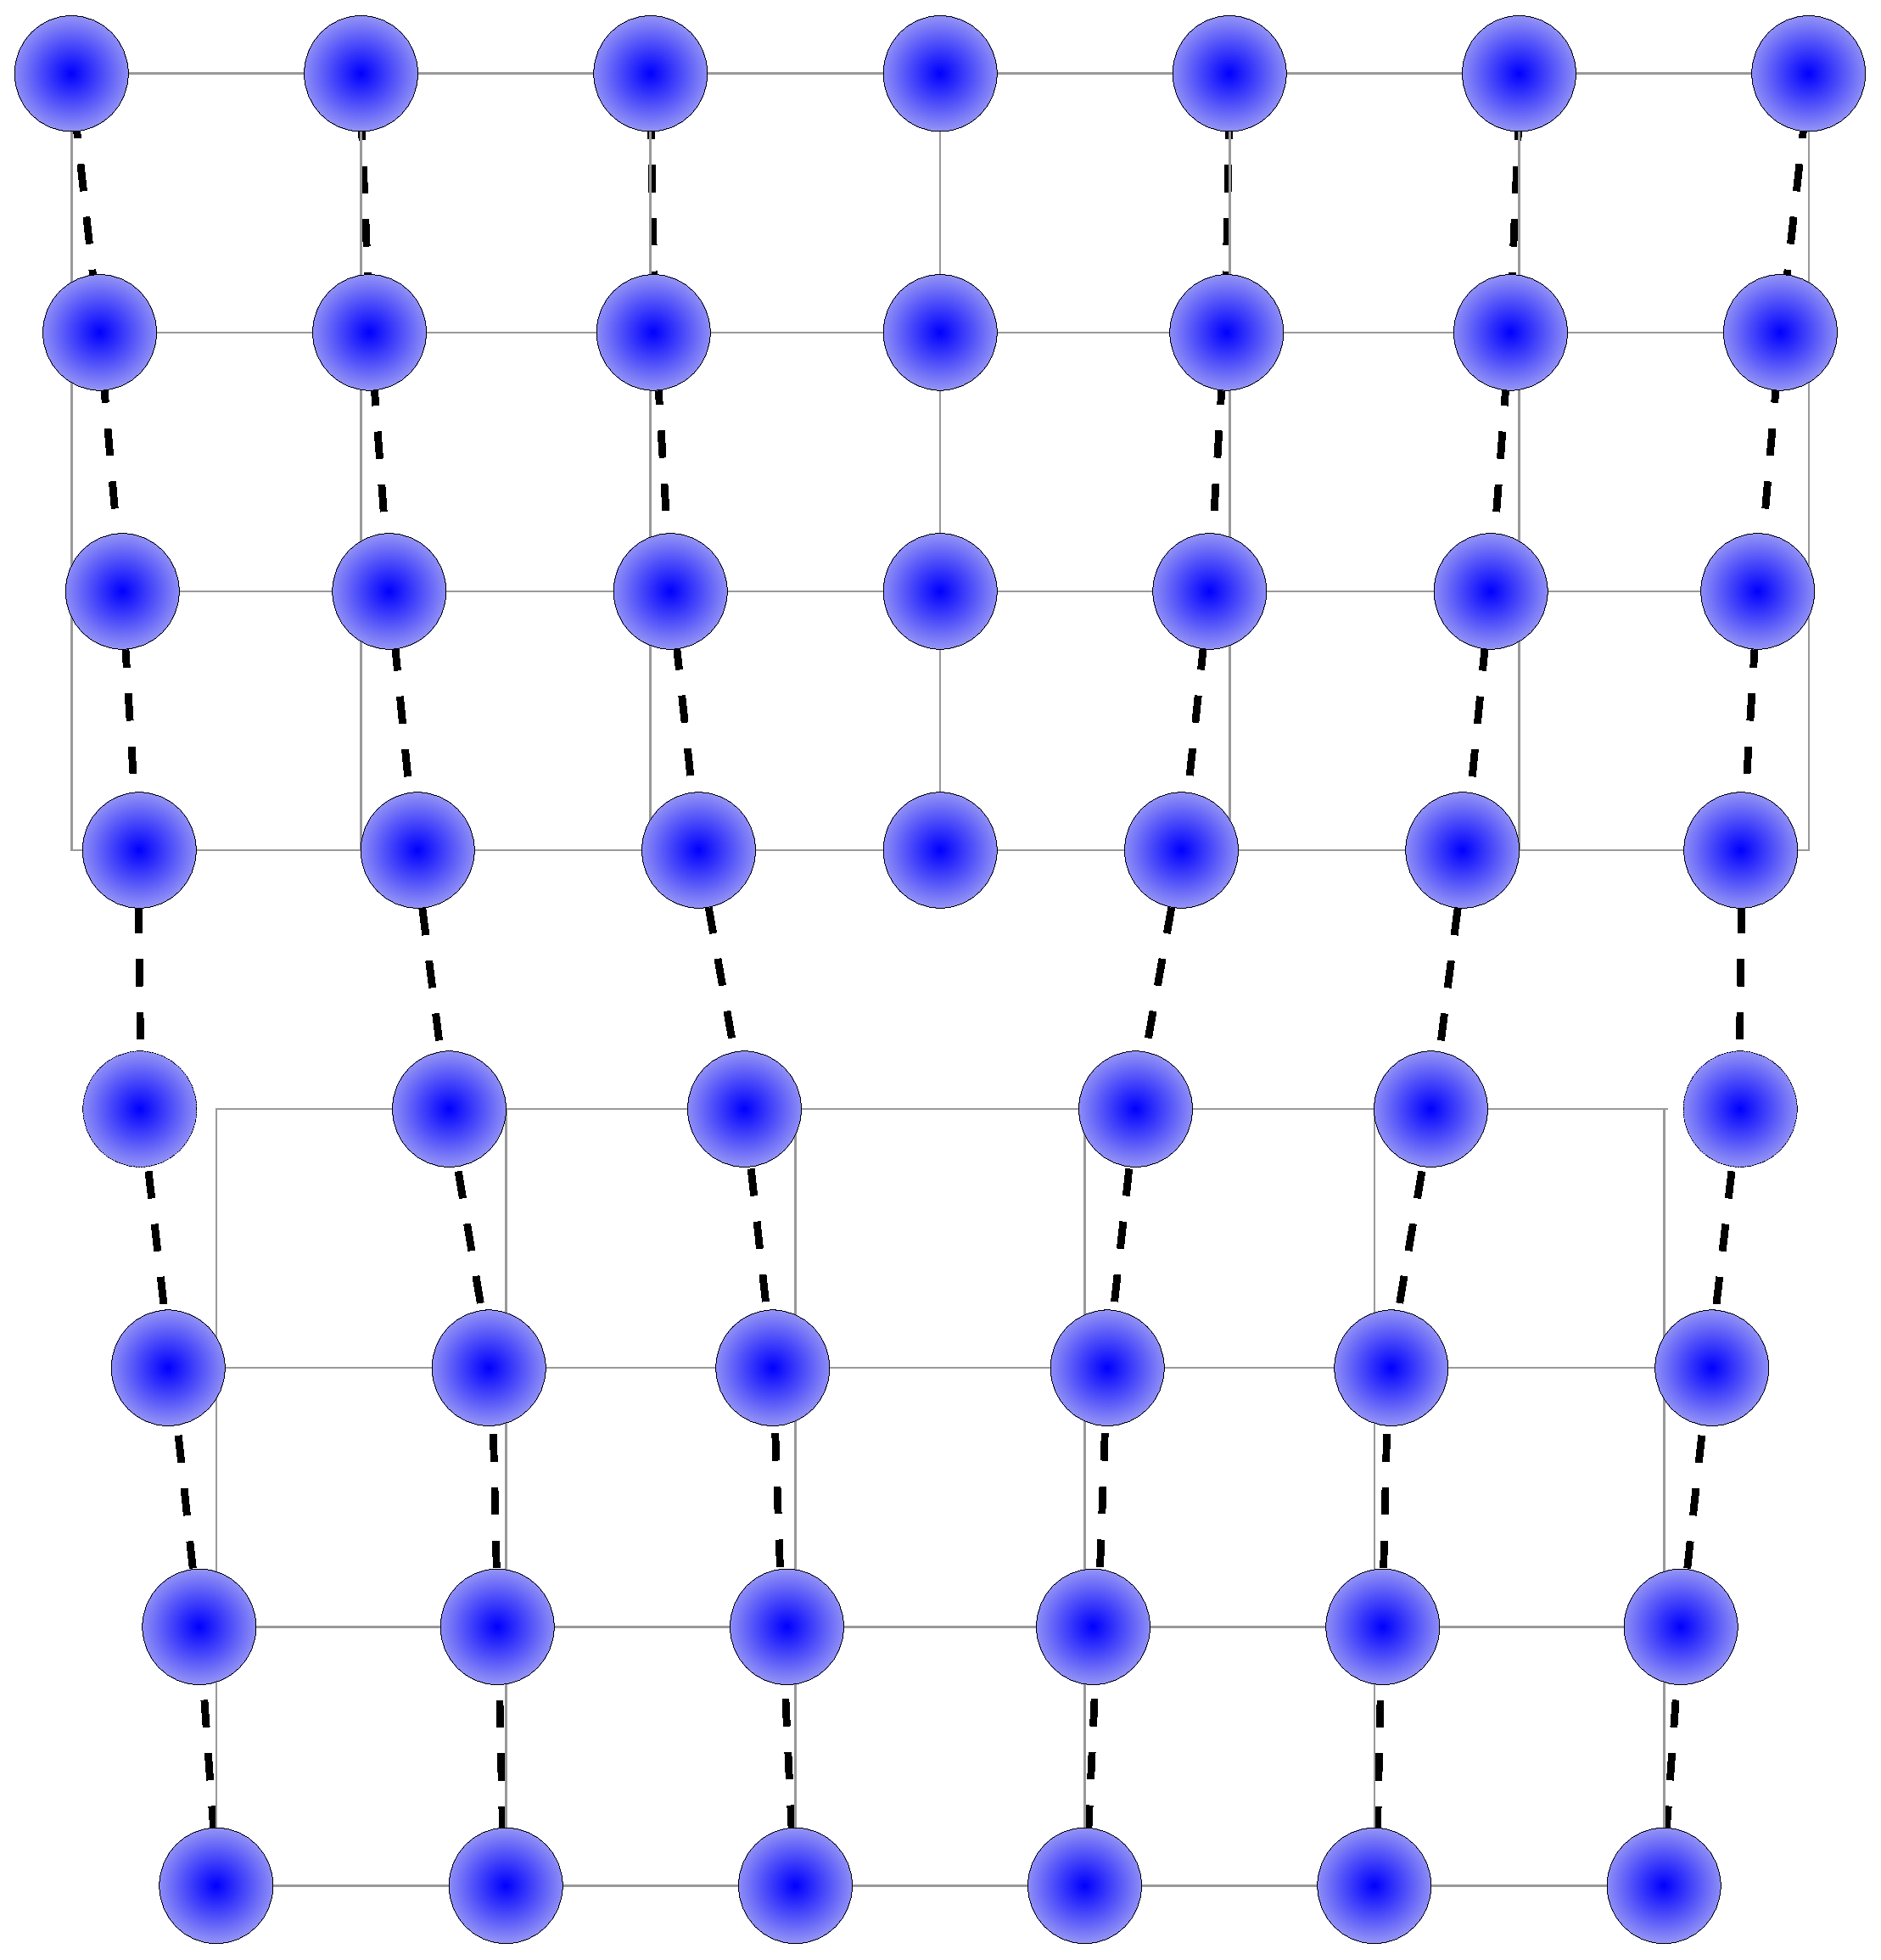
\includegraphics[width=\textwidth]{Edge_Dislocation}
        \caption{A schematic edge dislocation\label{fig:joined_half_crystals}}
    \end{subfigure}

    \caption{Schematics showing the creation of an edge dislocation in a simple square lattice by the joining of two misaligned half crystals. \label{fig:edge_disloc}}
\end{figure}



The Peierls model then estimates the energy of the configuration by considering two restoring forces generated by the atomic arrangement. These are shown in \autoref{fig:detail_of_peierls}. 

There are two forces that arise; firstly the bonds parallel the slip plane will be either extended or contracted, for example the bond between atom $A$ and $B$ has been contracted by the amount $\delta$, this will tend to oppose the concentration of misalignments to the core and  is zero in the case of no displacements from the initial positions; secondly the misalignment of bonds across the slip plane, the bond between atom $B$ and $C$ is misaligned by a lateral distance of $\phi$. This misalignment energy will tend to favour the concentration of the misalignments to the core and is a maximum in the case of no displacement from the initial position.


\begin{figure}
\centering
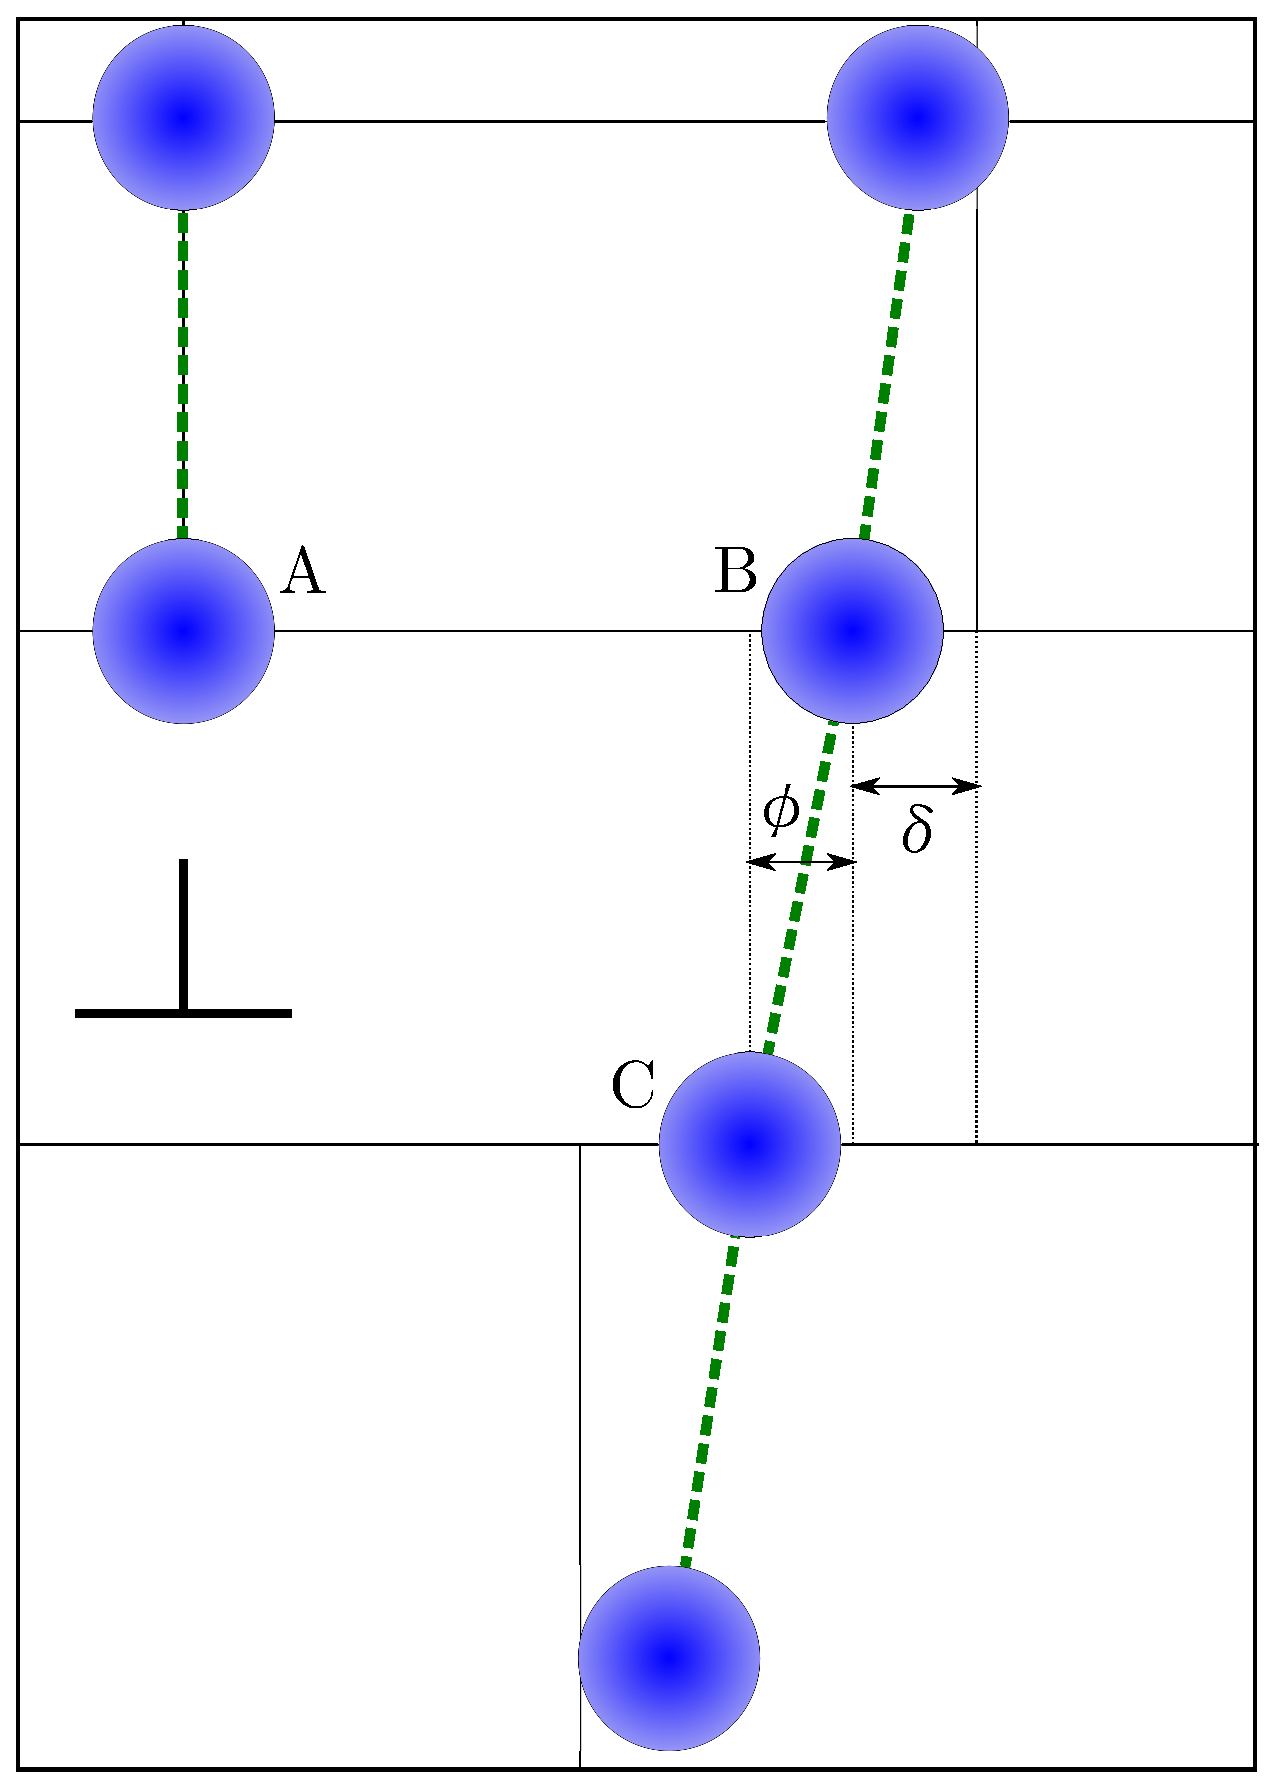
\includegraphics[width=0.6\textwidth]{peierls_model_detail}

\caption{Detail of the local displacements around the dislocation core. $\delta$ is the extension of the bond paralell to the slip plane while $\phi$ is the misalignment of the bond across the slip plane.\label{fig:detail_of_peierls}}
\end{figure}


The energy of the dislocation is the sum of all these contributions. This gives rise to a size, or width, of a dislocation. The width of the dislocation is defined as the distance from the core at which the misalignment across the slip plane is half its maximum, which occurs at the core. Peierls calculated this for an isotropic elastic solid and accounting for only the atomic planes immediately adjacent to the slip plane and found it to be 

\begin{equation}
w = \frac{d}{1-\nu}
\label{eqn:width_isotropic}
\end{equation}
where $d$ is the plane spacing across the slip plane and $\nu$ is the Poisson ratio.


Peierls gave the critical stress, now usually termed the Peierls Stress, for an isotropic elastic material, in terms of the ideal shear strength as calculated for uniform slip, as


\begin{equation}
\frac{\tau_p}{\tau_{ideal}} = \frac{4 \pi}{1 - \nu} (5.8 - \log|1-\nu|) \exp\left(-\frac{4\pi}{1 - \nu}\right).
\end{equation}

This was refined by \citet{Nabarro1947} and the direct summation of the discrete contributions was developed by Cottrell and Nabarro \cite{cottrell1953dislocations}. The result of that summation is



\begin{equation}
\tau_p = \frac{2\mu}{1-\nu} \exp\left( - \frac{4\pi w}{b} \right)
\end{equation}
where $\mu$ is the shear modulus and $b$ is the burgers vector.

For an isotropic material the width can be substituted from \autoref{eqn:width_isotropic}:

\begin{equation}
\tau_p = \frac{2\mu}{1-\nu} \exp\left( - \frac{2\pi d}{(1-\nu)b} \right).
\end{equation}

Although a simple model based on fairly large assumptions the method moved dislocation theory on in two ways: firstly continuum elasticity could not account for energy changes as the dislocation moves, this is the small difference between the continuous integral and discrete sum that depends on the core position, and secondly this approach removes the singularity at the core predicted by continuum elasticity for Volterra dislocations.


An important point to note here is the sensitivity of the Peierls stress to the size of the dislocation, $w$, or in the case of isotropic materials to the lattice geometry defined by $d/b$.


There have been many criticisms of and modifications to the Peierls model in the years since but these have largely focused on adjusting the assumptions of the original method.
In 1951 \citet{Foreman1951} introduced phenomenological potentials to describe the energy of the misaligned interactions across the slip plane, they discovered that the width of the dislocation was predicted to be larger than that of the original treatment and was coupled with a decrease in the Peierls stress. .
In 1955 \citet{Huntington1955a} modified the model to double the periodicity and so account for crystals in which a displacement of half a burgers vector is not symmetrical with no displacement, or in other words broke the mirror symmetry of the slip plane. 
\citet{Maradudin1959} considered a completely atomistic three dimensional model of a screw dislocation but did not consider radial displacements. That work only evaluated the energies of the symmetric and anti-symmetric configurations and so only estimated the energy change, not the maximum stress.



In 1994 a fully discrete model was developed by \citet{Ohsawa1994}. This model made similar assumption to the original Peierls model in that the only energy changes were in the sheared misaligned bonds across the slip plane but instead of solving for an analytical solution Ohsawa et al directly summed the energy of an atomic configuration that included 84 atoms, or 21 atomic spacing either side of the dislocation core. The model made no assumptions about the displacement field and instead iteratively improved all the atomic positions to find the equilibrium configuration. This was done for increasing applied external stresses until there was no stable configuration, i.e. slip would occur.



\citet{Bulatov1997} incorporated the concept of generalised stacking fault (GSF) energies into the Peierls model. This addresses a fault in the original Peierls formulation that the sinusoidal potential used to calculate the misalignment energy is too high and steep. \citet{Ohsawa1994} had already attempted to address this by using alternative potentials, but they were essentially arbitrary functions that fitted the shear modulus at small strains Instead Bulatov et al retained the variational approach but used density functional theory (DFT) calculations to generate a misalignment potential. They extended this to provide a three dimensional potential to allow both lateral and vertical displacements of the atoms in the slip plane. This is important around the core where large strains mean that the energy contributions are very inaccurate, and so by using the DFT to calculate a misalignment potential the Peierls model can bridge the length scales between the large scale stress and strain fields around the dislocation and the large local displacements at the core. This is no longer analytically solvable but is not difficult to solve numerically, the only limit being computational time.










